\chapter{Métodos}

% IM: Melhorar isso
Este trabalho prevê o desenvolvimento da ferramenta de documentação de implementação funcionalidades.

As etapas do estudo foram:

\section{Estudo de Aplicações Existentes}

Foi feita uma busca por aplicações que realizem atividades semelhantes a ferramenta proposta, ou seja, criação e compartilhamento de notas textuais. Dentre as ferramentas encontradas, seguem:

\subsection{Evernote}

Na época da elaboração deste trabalho, o Evernote\footnote{\url{https://www.evernote.com/}} era uma das ferramentas mais populares de criação de anotações privadas. Em 2014, atingiu a marca de mais de 100 milhões de usuários\footnote{\url{https://blog.evernote.com/blog/2014/05/13/evernote-reaches-100-million-users/}}. Ele possui um editor de texto com suporte a texto formatado, com listas, \textit{checkboxes}, \textit{\textit{links}}, anexos, tabelas. Os documentos criados na ferramenta (que possui clientes web, desktop e para diversas plataformas móveis) podem receber \textit{tags}, e ser colocados em pastas para melhor organização de modo a facilitar sua recuperação.

% IM: Mostrar uma anotação do evernote?

Documentos também podem ser compartilhados diretamente para outros usuários da ferramenta ou através de \textit{links} públicos (acessíveis para qualquer pessoa).

Dentre suas limitações para o uso para a redação de tutoriais da área de desenvolvimento de código está a falta de suporte a exibição de código com \textit{syntax-highlighting}, ou seja, com formatação apropriada.

% IM: Mostrar um exemplo de como código fica no evernote?

\subsection{GitHub e GitHub Gists}

Apesar de não ser sua principal proposta, o GitHub é muito utilizado por desenvolvedores para anotações, por possuir suporte a uma linguagem de marcação própria, chamada GitHub Flavored Markdown\footnote{\url{https://help.github.com/articles/github-flavored-markdown/}}. Esta linguagem funciona de maneira semelhante a outras do mesmo tipo como HTML ou LaTeX, permitindo que seus usuários escrevam textos apenas informando que determinadas seções do texto possuem tal significado como ``Título'', ``Lista'', entre outros.

Estas anotações normalmente são utilizadas em arquivos ``Leia-me'' de projetos e descrevem informações relevantes sobre estes (instalação, como executar testes, como fazer uso do projeto, etc).

\begin{figure}[h]
	\centering
    \caption{Exemplo de arquivo ``Leia-me''}
    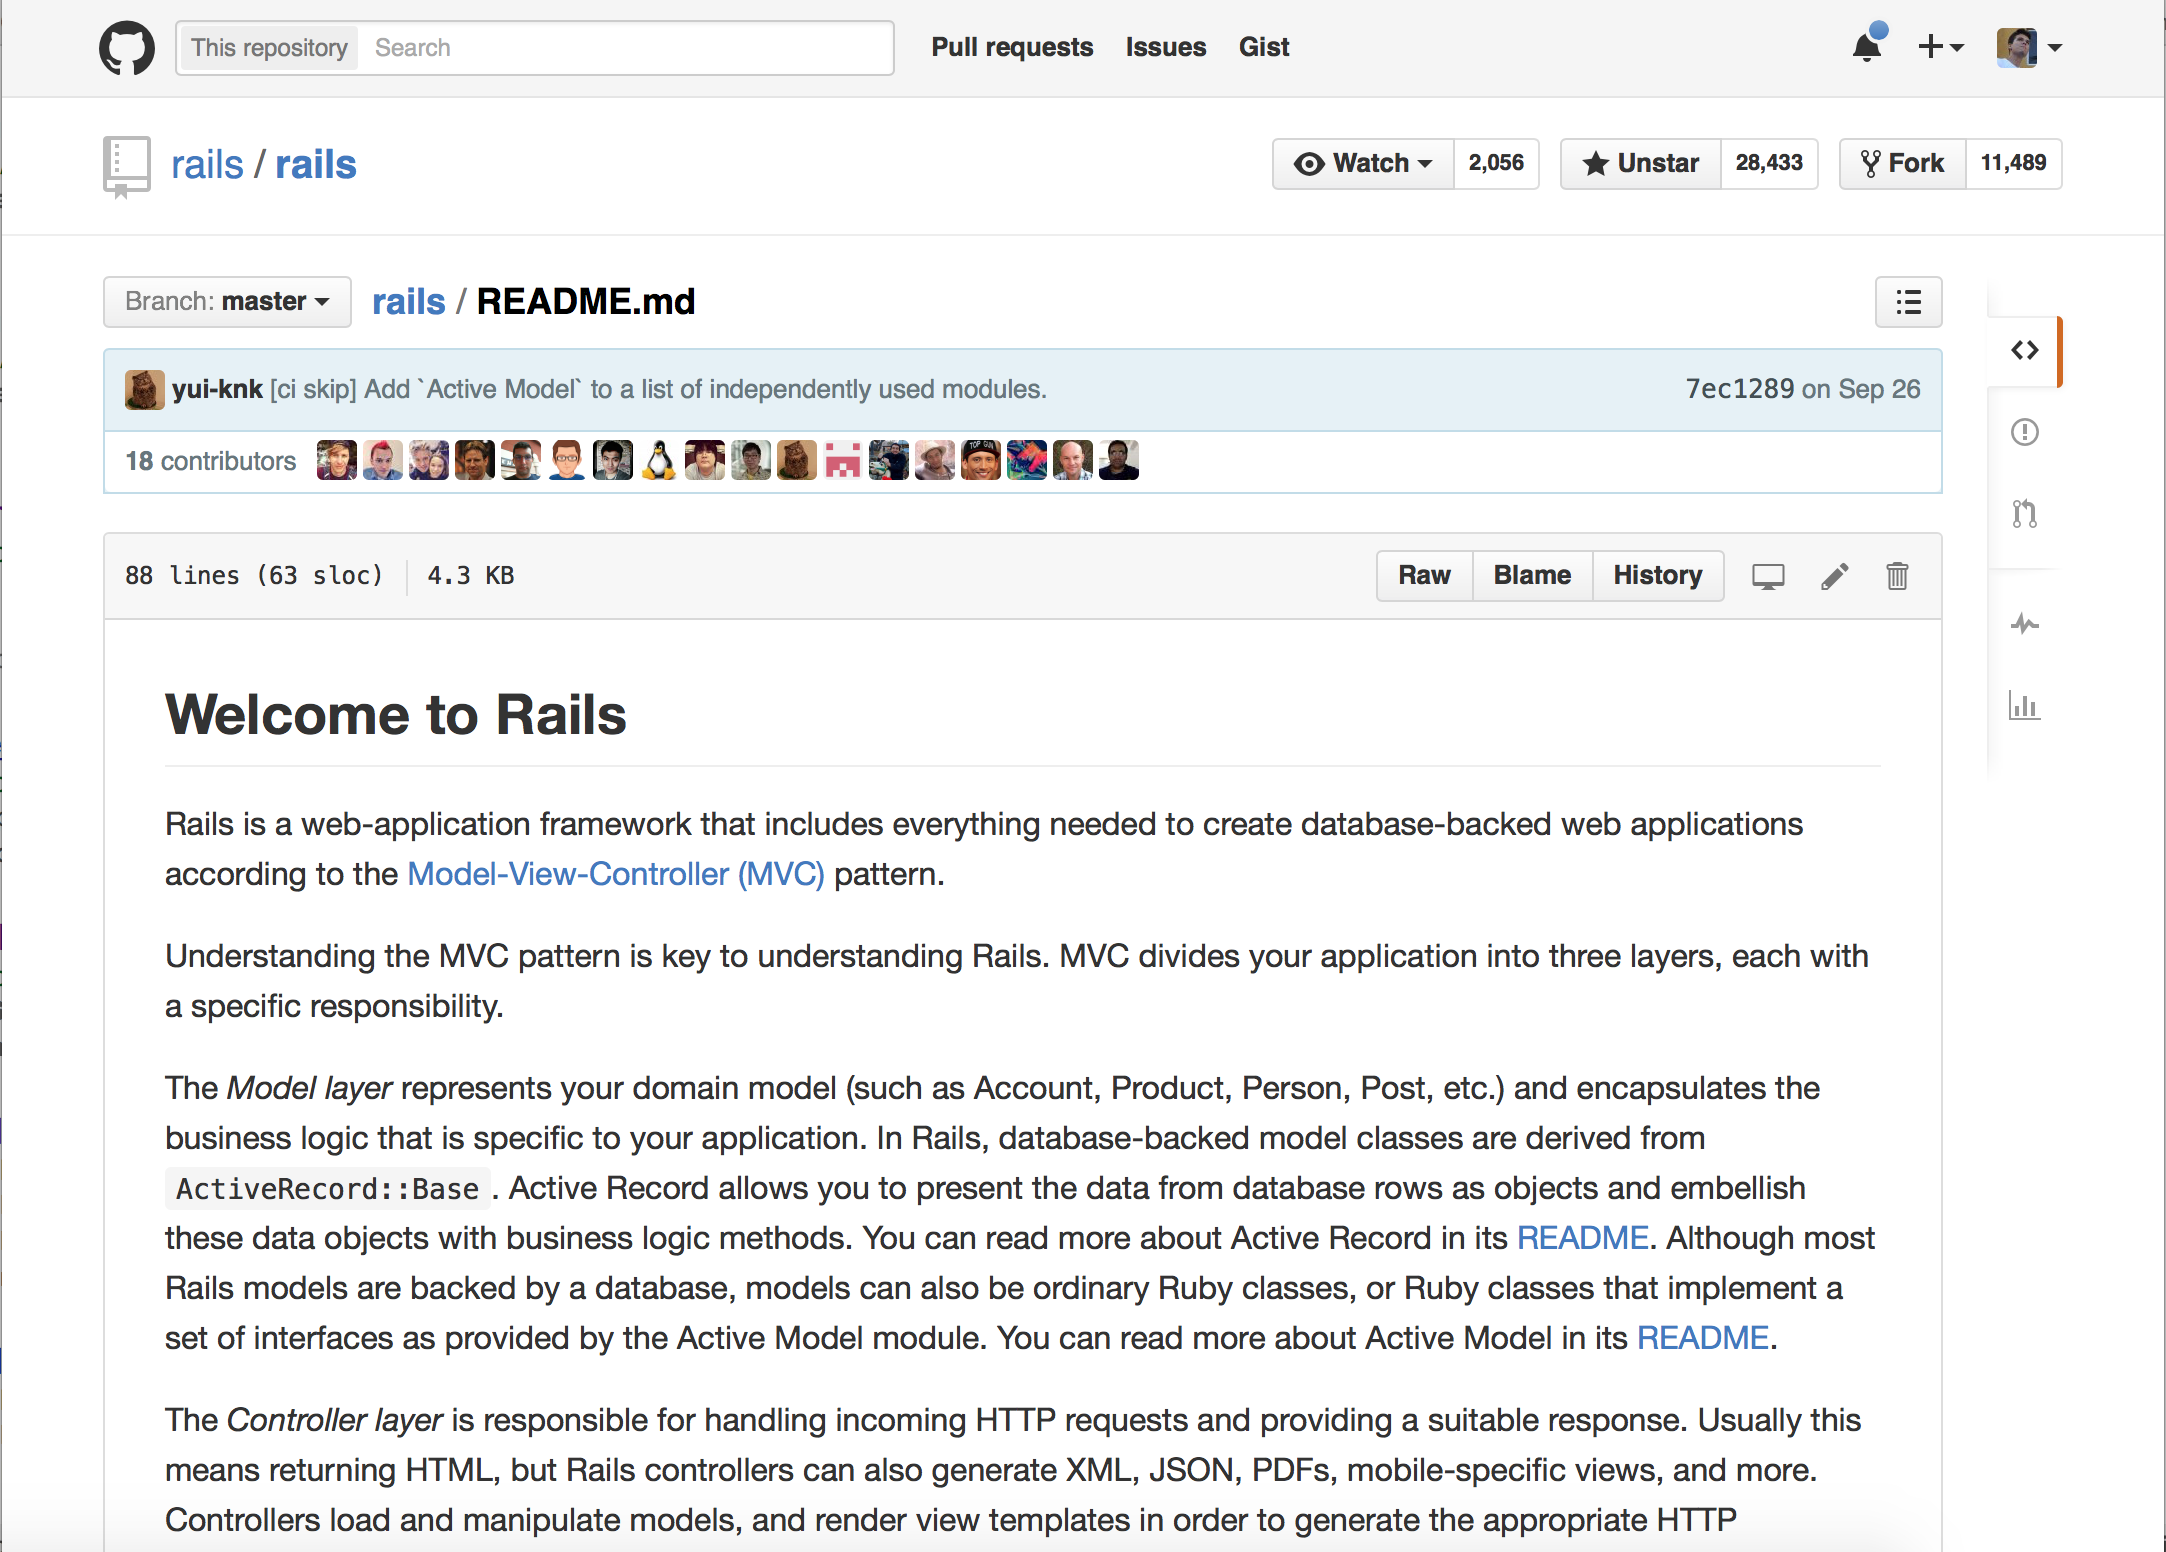
\includegraphics[width=15cm]{Imagens/print-readme.png}
	\caption*{Fonte: O autor (2015)}
\end{figure}

% https://github.com/rails/rails/blob/master/README.md
% IM: a imagem é daí. Essa é a fonte ou ainda sou eu?

Outra forma de se registrar anotações no GitHub é através de Gists\footnote{\url{https://gist.github.com}}. A comunidade de desenvolvimento de software comumente utiliza estes arquivos para registrar pequenos \textit{snippets} ou \textit{scripts} de código, com pouca ou nenhuma descrição sobre o mesmo.

Gists pertencem a somente um usuário (podendo ser públicos ou privados) e também possuem suporte a GitHub Flavored Markdown.

Vale notar que esta linguagem de marcação possui suporte a \textit{syntax-highlighting}, formatando código de maneira clara.

% IM: mostrar um exemplo de código com markdown aqui?

Dentre as limitações das ferramentas acima citadas, está a precária indexação (repositórios do GitHub e Gists não possuem \textit{tags}) dificultando a recuperação de informação relevante ao usuário.

% IM: tá fraca essa parte das limitações?

\subsection{Blogs e sites}

Uma das maneiras mais populares por desenvolvedores de se compartilhar tutoriais sobre questões de desenvolvimento são os \textit{blogs} de autoria própria.

Implementados em diversas tecnologias, possuem a vantagem de muitas vezes estarem indexados por ferramentas de busca como Google\footnote{\url{www.google.com}} e Bing\footnote{\url{www.bing.com}}.

Além disso, existem uma série de \textit{plugins} em diversas tecnologias que permitem a escrita de texto tanto em linguagens de marcação como WYSIWYG (\textit{What You See Is What You Get}, ou seja, ``O que você vê é o seu resultado''), se assemelhando a editores de texto como Microsoft Word\footnote{\url{https://products.office.com/en-us/word}} ou Pages\footnote{\url{http://www.apple.com/mac/pages/}}. Alguns destes \textit{plugins} possuem inclusive suporte a visualização de código com \textit{syntax-highlighting}.

Porém, muitas vezes estes \textit{plugins} possuem problemas para renderizar código que foi copiado de alguma outra fonte (como de arquivos de algum repositório do GitHub, por exemplo). Por exemplo, o \textit{plugin} utilizado no website de perguntas e respostas de programação Stack Overflow exige que todo texto que representa código seja identado utilizando quatro espaços. Códigos de aplicações desenvolvidas na linguagem Ruby, por convenção de estilo, geralmente estão identados utilizando somente dois espaço. Assim, quando se copia e cola código já pronto desta linguagem, o editor de texto exibe um aviso exigindo a formatação correta do código para renderização correta. O redator então deve, linha por linha, alterar a quantidade de espaços dados, demandando de esforço e tempo.

\bigskip

Dessa forma, levou-se em consideração as limitações e pontos fortes de cada uma das ferramentas analisadas durante a elaboração da ferramenta deste trabalho.

\section{Inquérito contextual}

A partir da etapa anterior, o estudo para a concepção da ferramenta passou a levar em consideração requisitos e necessidades de desenvolvedores de software. O processo está descrito a seguir.

\subsection{Contexto}

Para a elaboração da ferramenta, houve participação da equipe de desenvolvedores da empresa júnior\footnote{\url{http://en.wikipedia.org/wiki/Junior_enterprise}} 4Soft\footnote{\url{http://www.4softjr.com.br}}. A empresa é vinculada aos curstos de Bacharelado em Engenharia de Software\footnote{\url{http://www.dimap.ufrn.br/pt/graduacao/engenharia-de-software/apresentacao}} e Bacharelado em Tecnologia da Informação\footnote{\url{http://www.imd.ufrn.br/curso_bacharelado.php}} da Universidade Federal do Rio Grande do Norte (UFRN)\footnote{\url{http://www.ufrn.br}}. A empresa atua na área de desenvolvimento de software web para clientes de diversos ramos (em geral pequenos e médios negócios) e é formada exclusivamente por alunos dos cursos citados.

O autor do trabalho atua na empresa há três anos e meio, atuando em atividades de gerência de equipes e mentoria de novos membros, além de na própria área de desenvolvimento de software. Nesse período, passaram pela empresa cerca de dezessete desenvolvedores com nível de conhecimento variado. Participaram do estudo oito desenvolvedores com experiência em média de dois anos na empresa.

Além disso, o \textit{chat} utilizado por uma turma de Desenvolvimento de Sistemas Web ofertada no primeiro semestre de 2014 para alunos dos cursos de Bacharelado em Engenharia de Software e Bacharelado em Ciência da Computação foi analisado. A turma possuia um total de vinte e cinco alunos e seu projeto final envolvia a participação de todos colaborativamente sobre um mesmo projeto. A maioria dos alunos possuia pouca ou nenhuma experiência com a tecnologia utilizada na disciplina.

\subsection{Inquérito}
% IM: Coloco este título mesmo?

Entrevistas não estruturadas e seções de \textit{brainstorm} foram feitas pelo autor com cinco participantes da empresa júnior mencionada. Além disso, por ser membro da empresa, o autor pôde observar o funcionamento interno da equipe. Procurou-se entender como se dava o fluxo da resolução de uma dúvida que algum desenvolvedor apresente.

Foi feita a análise das perguntas postadas no \textit{chat} utilizado pela empresa no último ano bem como o \textit{chat} utilizado pelos alunos da disciplina de Desenvolvimento Web. Pôde-se concluir que as dúvidas postadas geralmente se enquadravam em alguma das seguintes categorias:

\begin{enumerate}
  \item \textbf{Como}. Instruções sobre implementar uma determinada funcionalidade ou ação.
  \item \textbf{Tomada de decisão}. Qual a melhor maneira de realizar determinada implementação.
  \item \textbf{Revisão de código}. Revisão de alguma implementação já feita.
  \item \textbf{Erro}. Ajuda com a resolução de algum \textit{bug} com mensagem de erro claramente fornecida.
  \item \textbf{Discrepância}. Solicitação de explicação sobre comportamento inesperado apresentado pelo código.
\end{enumerate}

Cujos trechos de conversas extraídas do \textit{chat} da empresa júnior ao longo deste trabalho e anexos exemplificam.

\begin{figure}[h]
	\centering
    \caption{Dúvida do tipo 1}
    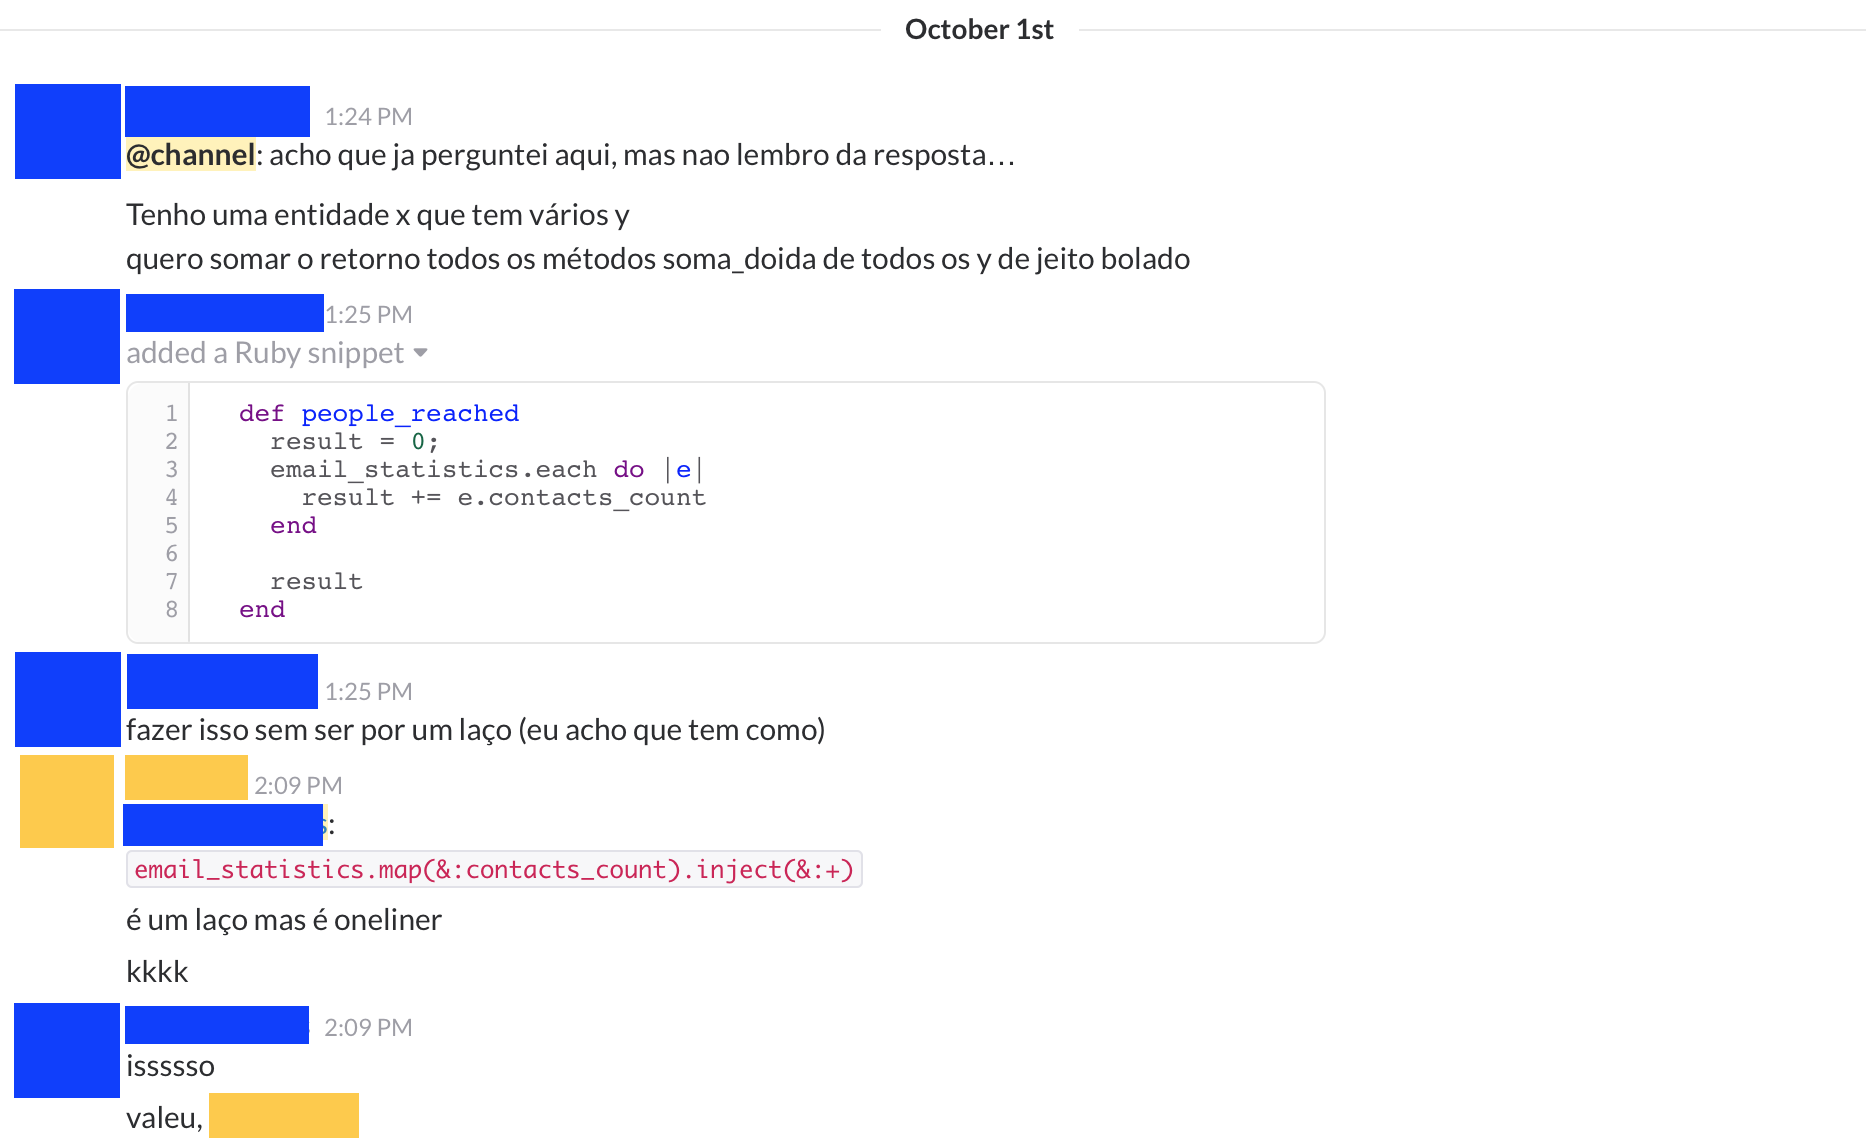
\includegraphics[width=15cm]{Imagens/c-type-1-9-1.png}
	\caption*{Fonte: Adaptado de Slack (2015)}
\end{figure}

\begin{figure}[h]
	\centering
    \caption{Dúvida do tipo 2}
    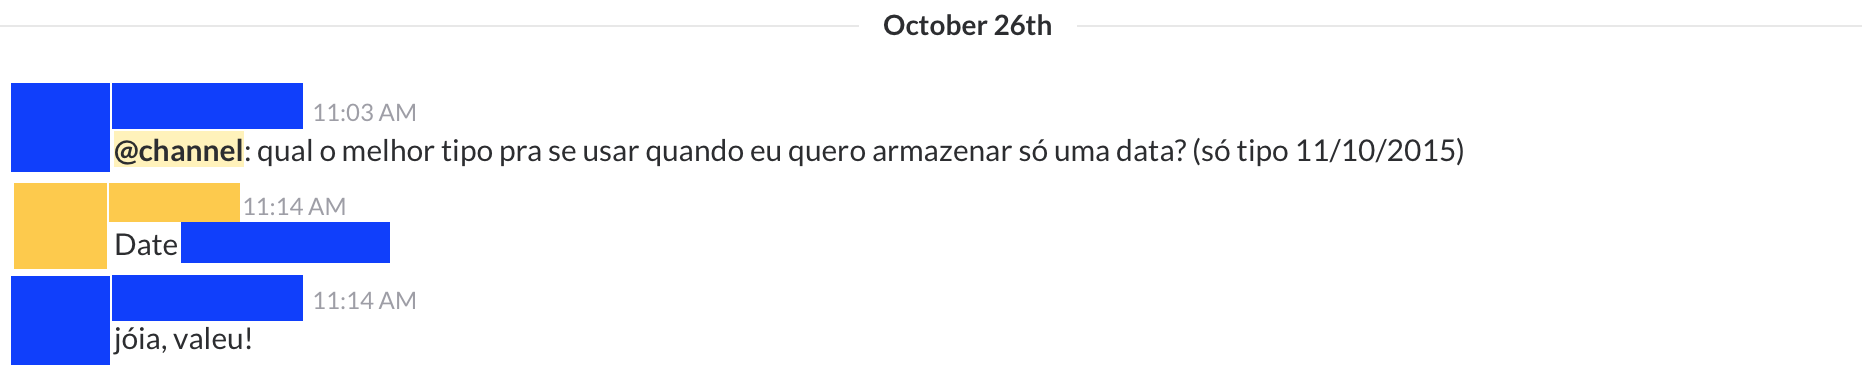
\includegraphics[width=15cm]{Imagens/c-type-2-1-1.png}
	\caption*{Fonte: Adaptado de Slack (2015)}
\end{figure}

\begin{figure}[h]
	\centering
    \caption{Dúvida do tipo 3}
    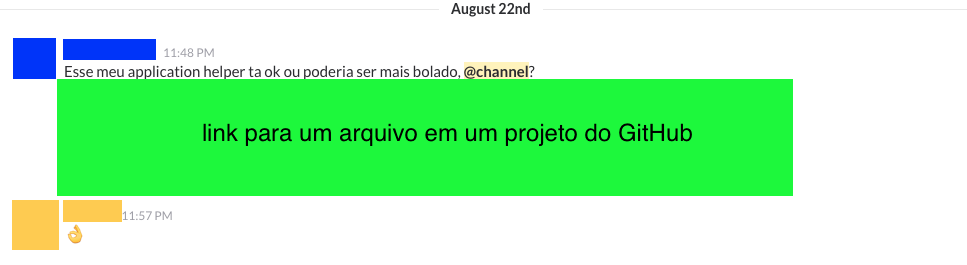
\includegraphics[width=15cm]{Imagens/c-type-3-1-1.png}
	\caption*{Fonte: Adaptado de Slack (2015)}
\end{figure}

\begin{figure}[h]
	\centering
    \caption{Dúvida do tipo 4}
    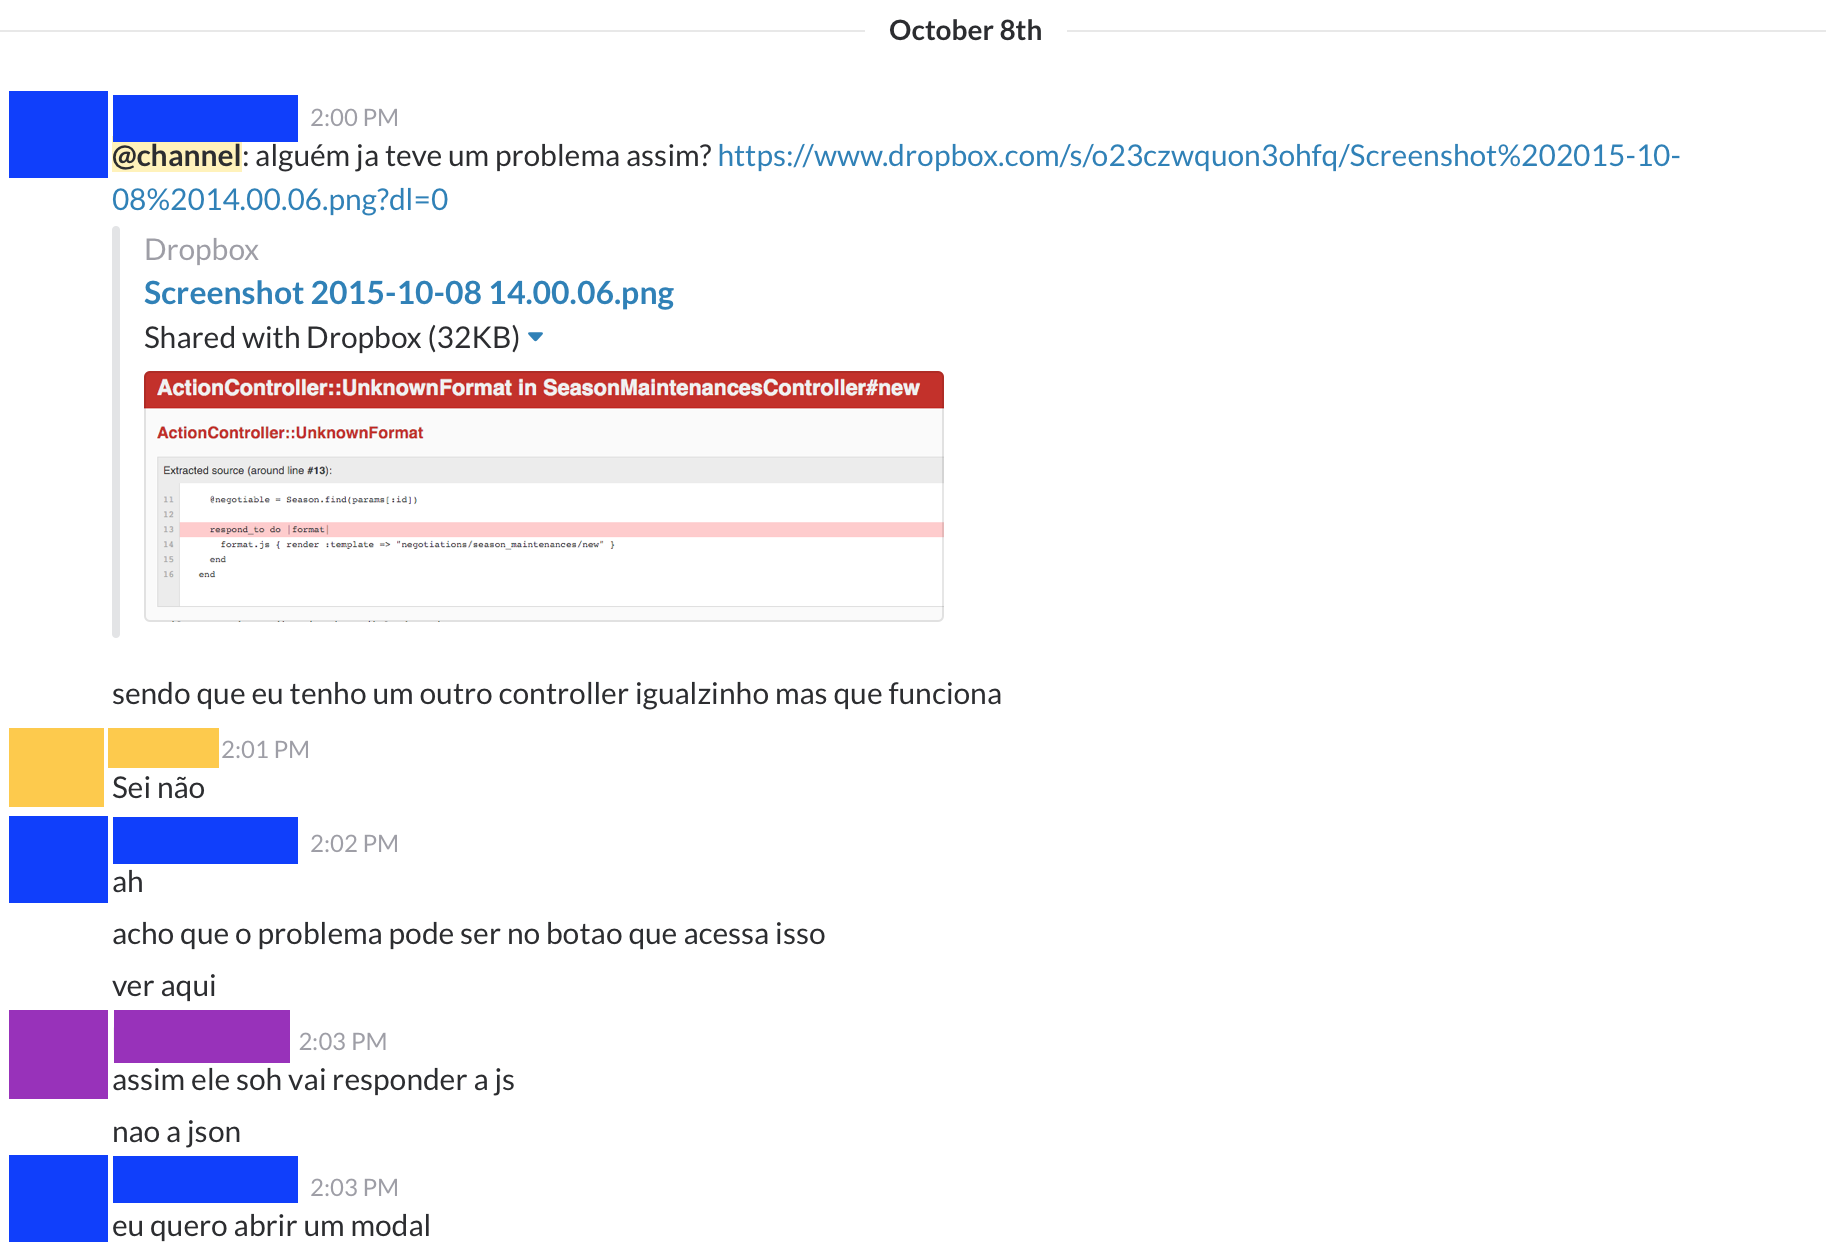
\includegraphics[width=15cm]{Imagens/c-type-4-1-1.png}
	\caption*{Fonte: Adaptado de Slack (2015)}
\end{figure}

\begin{figure}[h]
	\centering
    \caption{Dúvida do tipo 4 (continuação)}
    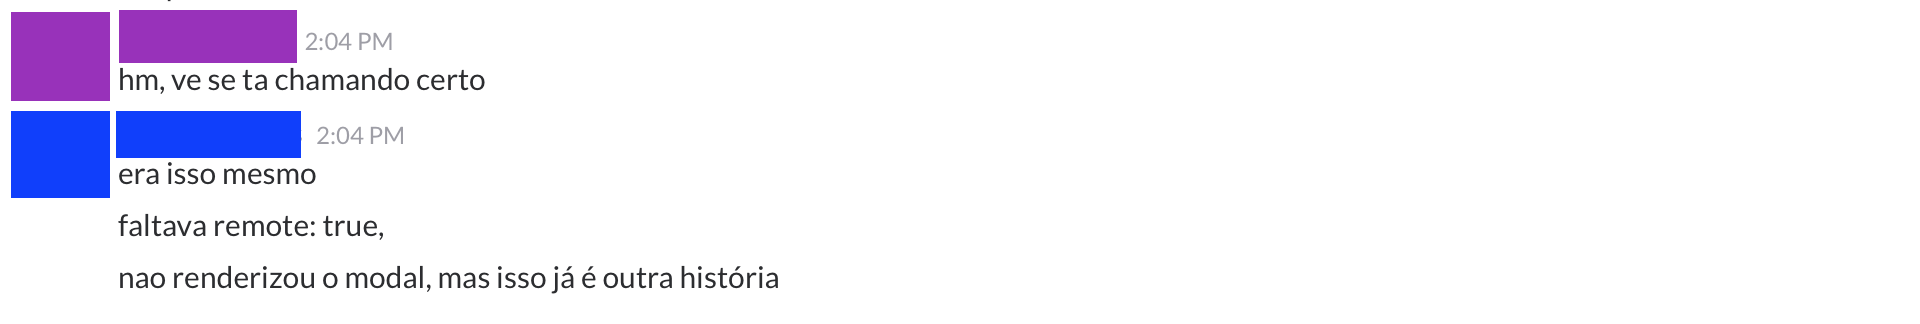
\includegraphics[width=15cm]{Imagens/c-type-4-1-2.png}
	\caption*{Fonte: Adaptado de Slack (2015)}
\end{figure}

\begin{figure}[h]
	\centering
    \caption{Dúvida do tipo 5}
    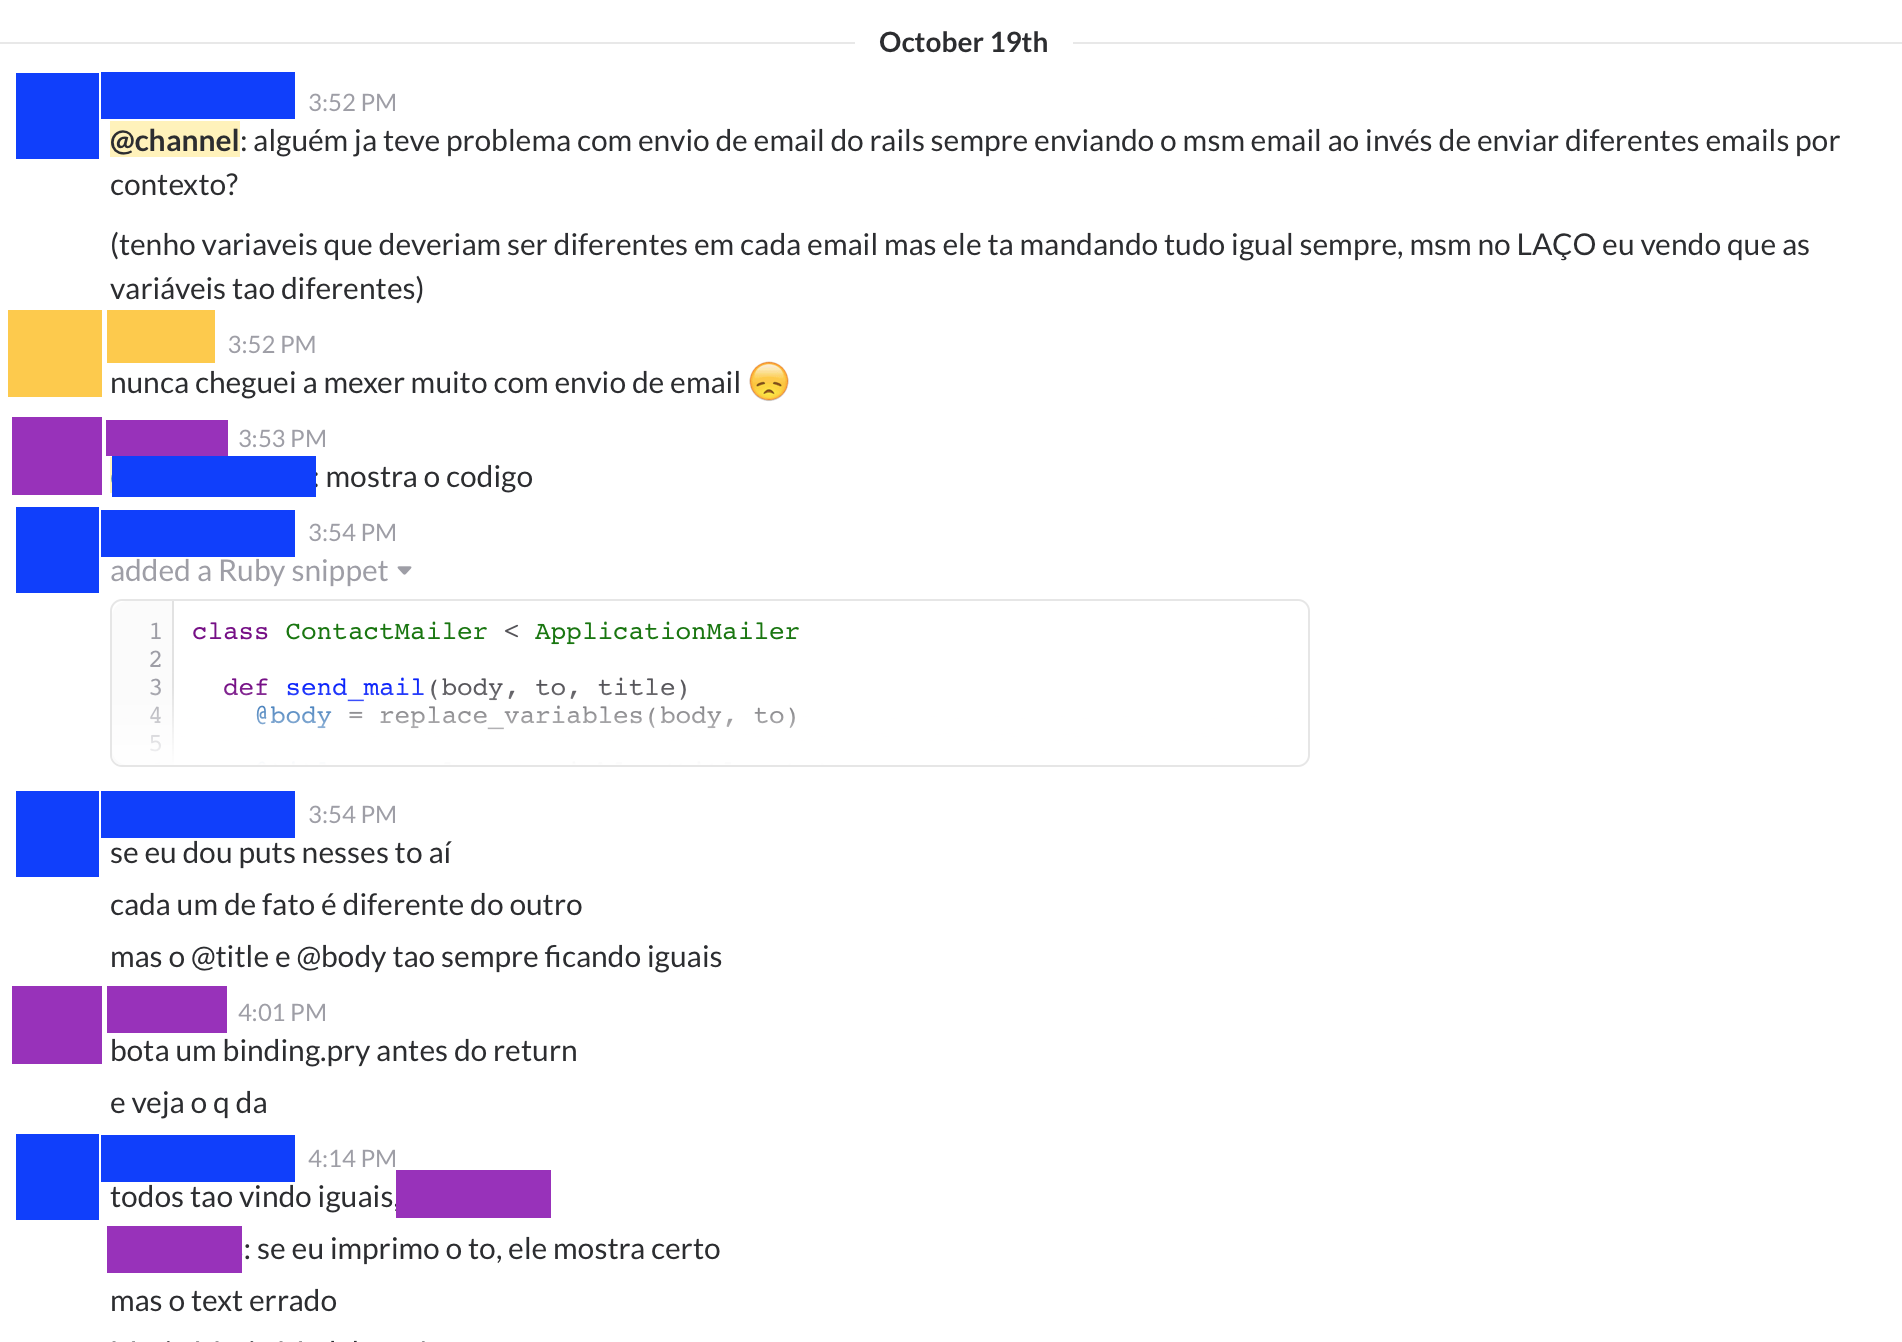
\includegraphics[width=15cm]{Imagens/c-type-5-2-1.png}
	\caption*{Fonte: Adaptado de Slack (2015)}
\end{figure}

% IM: descobrir como fazer essa citação
Estas categorias se enquadram dentro das dez categorias também encontradas por Treude et al.~\cite{Treude2011} em seu estudo sobre como desenvolvedores realizam perguntas no site de perguntas e respostas Stack Overflow.

Além da análise das perguntas realizadas pelos desenvolvedores, foi feita uma análise sobre como estas eram respondidas no mesmo período. Para todos os casos citados, o fluxo de resolução do problema se dava na maioria dos casos da seguinte forma:

\begin{enumerate}[i]
  \item O desenvolvedor comunicava o problema (para todos os membros ou somente um) no \textit{chat} utilizado pela equipe.
  \item Para todos os casos, um ou mais membros da equipe discutiam sobre como resolver a dúvida proposta e ofereciam uma solução. Em certos casos, exemplos de código eram fornecidos ou \textit{links} relevantes eram enviados.
  \item O desenvolvedor que comunicou o problema tentava implementar a funcionalidade utilizando as recomendações oferecidas.
  \item Caso novas dúvidas surgissem durante a implementação, os demais membros da equipe tentavam dar recomendações mais precisas ou oferecer outros exemplos e \textit{links} úteis.
  \item O problema era solucionado.
\end{enumerate}

Para casos em que a resolução problema encontrado não era de conhecimento de nenhum membro da equipe (seja por falta de contato com o contexto ou até mesmo por esquecimento), o desenvolvedor realizava pesquisas em ferramentas de busca para encontrar tutoriais ou fóruns de discussão que o ajudassem a resolver o problema.

Se tratando de esquecimento, desenvolvedores relataram que era comum que os próprios lembrassem que já enfrentaram determinado problema, mas não se lembram da solução que foi dada para tal. Isso era comum em especial em problemas do tipo 4. Erro.

Observou-se também que era frequente que a mesma pergunta fosse feita por um outro desenvolvedor após certo tempo e respostas semelhantes eram oferecidas (e inclusive os mesmos \textit{links} eram disponibilizados).

Desta etapa, concluiu-se que a ferramenta proposta deveria ser concebida levando em conta que:

\begin{itemize}
  \item Exemplos de código da própria equipe são importantes para a resolução de uma dúvida.
  \item Um bom sistema de recuperação deve existir, pois desenvolvedores apresentam as mesmas dúvidas mais de uma vez.
  \item \textit{Links} de tutoriais já prontos devem ser levados em consideração.
\end{itemize}

\section{Definição dos Requisitos da Ferramenta e Implementação}

Com base no Inquérito Contextual e Estudo de Aplicações Existentes, o autor pode elicitar os seguintes requisitos para uma ferramenta que diminua os esforços com mentoria/ resolução de dúvidas de desenvolvedores:

\begin{itemize}
  \item A ferramenta deve agir como um catálogo de anotações/ documentos feitos pela equipe.
  \item Deve haver o suporte a exibição de código (da própria equipe) e com formatação apropriada.
  \item Um bom sistema de recuperação de informações deve se fazer presente.
  \item Links de tutoriais já prontos devem ser levados em consideração.
\end{itemize}

Com base nisso, partiu-se para a implementação da ferramenta, denominada Twydi (um acrônimo para ``\textit{That's the Way You Do It}'', em português: ``É assim que se faz''). O detalhamento sobre este processo e das funcionalidades apresentadas por esta se encontram no próximo capítulo.

\section{Implantação, Observação do uso da Ferramenta e Aplicação de questionário}

A ferramenta então foi disponibilzada em dois servidores diferentes: um para uso da empresa júnior e de outros interessados e outro para uso dos alunos da disciplina de Desenvolvimento Colaborativo de Software ocorrida no segundo semestre de 2015. Os artefatos gerados em um servidor não estavam disponíveis no outro. Ao todo, quatorze artefatos foram produzidos ao longo de três semanas por dez diferentes autores, sendo sete artefatos produzidos por três membros empresa júnior e sete produzidos por sete membros da disciplina em questão. Foram obtidas oito respostas no questionário aplicado, sendo duas por membros da empresa júnior e as demais por alunos da disciplina. Ao todo o questionário possuia quinze perguntas e se encontra nos anexos do trabalho.

% IM: Verificar se já falei da disciplina antes desse parágrafo
% IM: verificar se quantidade de perguntas está correta
% IM: acredito que meus twydies estejam no meio dessas contas, bem como eu estou na quantidade de usuários. Preciso me excluir?
